\documentclass[a4paper]{article}
\usepackage{graphicx}
\usepackage{onecolceurws}
\usepackage{csquotes}
\usepackage{hyperref}
\usepackage{framed}
\usepackage{mdframed}
\usepackage{upquote}
\usepackage{lmodern}
\usepackage[normalem]{ulem}

\newcommand\todo[1]{\textcolor{red}{TODO: #1}}

\title{Sophize Knowledge Organization}

\author{ Abhishek Chugh }

\graphicspath {{../res}}

\institution{ Sophize Foundation\\ Bengaluru, India \\ abc@sophize.org }

\begin{document}
\maketitle

\begin{abstract}
Sophize is a novel mathematics library and discussion platform with a mission to help our users find and organize mathematical proofs. We present Sophize's novel yet familiar knowledge organization scheme that is used to represent a wide variety proofs. With this knowledge organization scheme at its core, we have engineered a platform to aggregate knowledge from multiple sources. The platform meaningfully combines knowledge from published research, encyclopaedias such as PlanetMath and Wikipedia, informal computer programs and formal systems such as Metamath; and allows its users to run a federated search over them. To make this happen, two developments were necessary. First, we developed an open plugin architecture that allows proofs from computer programs to be generated as required. Second, we extended the Markdown language to represent the connections between between mathematical objects found across various sources of knowledge. In addition, we also utilized this new language to create a novel communication system built specifically to aid mathematicians in solving problems collaboratively.

\end{abstract}

\vskip 32pt

\section{Introduction}

\subsubsection*{Background: The Sophize Platform}

- The goal is rational truth. Three dimensions are consistency, correspondence and values.

- No hidden assumptions. Should have clear answer to every question of the form `why do you believe X'.

- In its current iteration, Sophize implements consistency. Knowledge represented by manually and automated generation of arguments. Can model vast majority (almost all) of mathematics.

- This gives you a way to create (consistency enforced) models. Next step is to see how accurately these models represent (parts of) the World. That involves quantifying correspondence of observations with the predictions made by the theories.

- And finally, you need model individual, institutional, and societal values to claim the truth of `ought statements' like `I should wear a mask' or `Masks should be mandated'.

- These starting beliefs (axioms, principles, laws, assumptions) and values are a way to model our belief systems. There are no absolutes, each belief system results in a different rational truth.



\subsubsection*{Proofs in Sophize}
Sophize is a novel mathematics library and discussion platform. The author has developed the platform over the course of the last two years at \url{https://sophize.org}. Sophize's primary mission is to help users find existing proofs of mathematical statements, to discover new proofs, and to utilize this knowledge in their work. We combine knowledge from multiple resources and have accumulated thousands of definitions, theorems, and proofs from a wide variety of sources, including some published research, the PlanetMath encyclopaedia, Wikipedia, and the Metamath formal system \cite{metamath}.


Mathematical proofs are based on a variety of foundations such as ZFC, intuitionistic logic, and type theory. The arguments used in any proof are considered valid or not based on criteria that can vary. Most academic mathematics is peer-reviewed and published, but some mathematical proofs can be found in community curated sources such as Wikipedia. Proofs can also be algorithmically generated, and at the highest level of verification, they are represented and verified using a formal system. 

Sophize combines such an expansive range of proofs into a dense graph of propositions and logical arguments that aggregates knowledge from several documents and other data sources. We use this graph and combine it with the set of foundations and verifications chosen by each user to create proofs tailored to their needs. This introductory video gives an overview of the platform's offerings: \url{https://youtu.be/Wb1JbW9Otek}.

\begin{figure}[htbp]
\begin{center}
\fbox{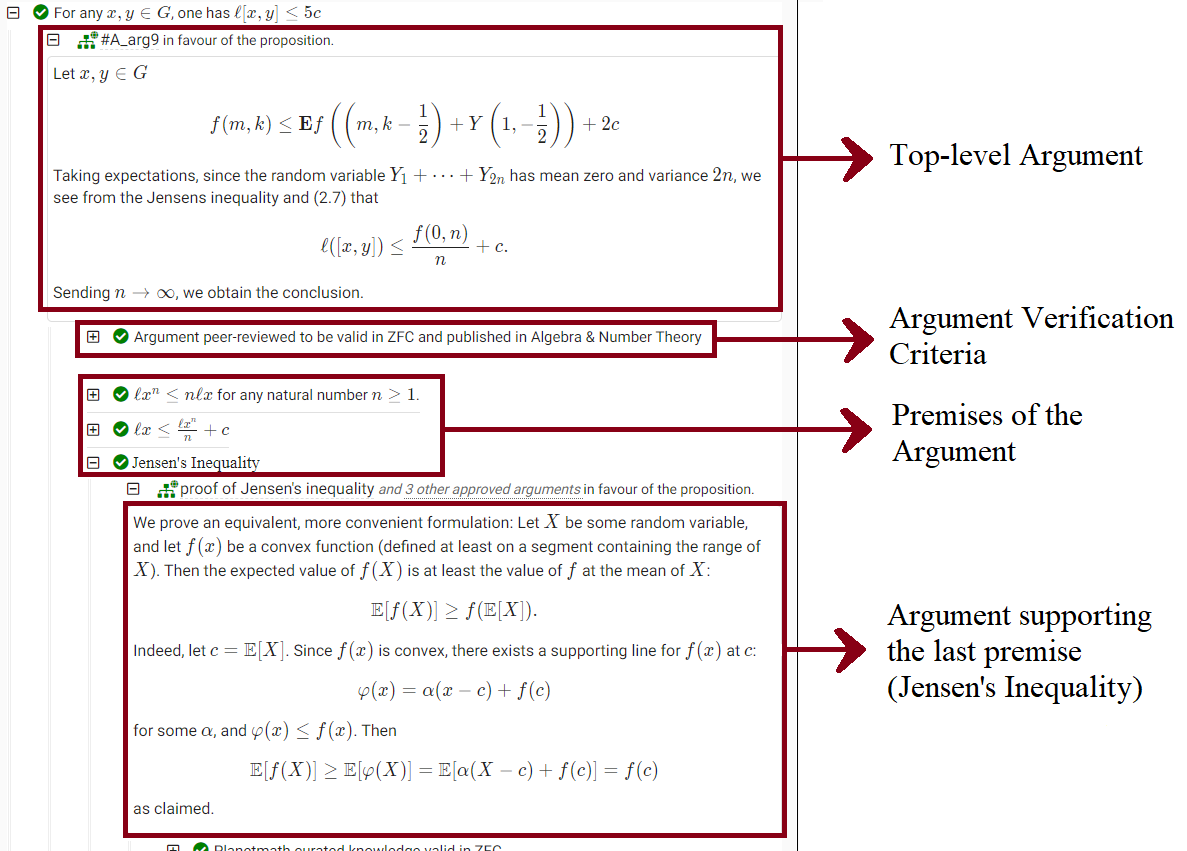
\includegraphics[height=12cm]{proof_tree}}
\caption{A proof displayed as a graph (tree) of arguments and propositions on the Sophize platform.}
\label{proof_tree}
\end{center}
\end{figure}

This work can also be seen as a step towards formalizing the network of information that exists in the connections of mathematical objects. The committee on planning a global library of the mathematical sciences recognized that this network is largely unexplored, and formalizing it has tremendous potential to accelerate math research \cite{sciences2014developing}.

Hence, we required novel knowledge organization techniques to connect mathematical entities from such a wide range of formal and informal knowledge sources. And thus, one of the main challenges towards building the Sophize platform was to create a simple way to embed mathematical entities on the web. \todo{Explain and summarize the problem statement}


\subsubsection*{Contribution}
\todo{summarize sections. section 3 does X, section 4 does Y etc.}


\section{Sophize's Knowledge Organization Scheme}
At its core, Sophize's approach is to simply keep track of all arguments in favour or against any proposition. Use of some form of arguments is the common factor amongst all mathematical (and perhaps all scientific) knowledge. We use this fact to unify knowledge from multiple sources in a meaningful way as described below.

We use the set of all known arguments to track knowledge from a variety of foundational theories. For theoretical knowledge, i.e., knowledge that doesn't involve empirical data, the primary criteria of validity is internal (logical) consistency. Thus, for each foundational theory (`belief set' described below), we also keep track of any contradictions that arise from those foundations.
\todo{section is crap, overview of how aggregated}

\subsection{Core Concepts}
Sophize uses the following concepts to logically organize theoretical knowledge.

\paragraph{A \textbf{resource} is an abstract concept inherited by all other top-level concepts like terms, propositions, arguments, and belief sets. Each resource has a URI and contains fields such as search tags and citations.}

A \textbf{URI} consists of two parts: a namespace-like identifier called its dataset-id, which indicates the data source, and a resource-id that specifies the resource type and its unique name in the data source. The dataset-id may be omitted if it can be inferred from the surrounding context.

For example, the Pythagorean theorem (a \textbf{P}roposition) represented in the Metamath project may have the URI \emph{metamath/\textbf{P}\_pythagorean} and the definition of cone (a \textbf{T}erm) extracted from Wikipedia may have the URI \emph{wiki/\textbf{T}\_cone}. When used inside another resource in the same (`wiki') dataset, cone's definition can be referred to simply as \emph{T\_cone}.

The same URI scheme will be used in this paper to refer to various terms, propositions, arguments, etc.

\paragraph{A \textbf{term} is a clearly defined entity that can be used to make up a valid proposition. It can be a mathematical object, operator, symbol, data structure, algorithm, or even a person. `Meaningless' primitives in formal theories are also categorized as terms.}

\paragraph{A \textbf{proposition} is a grammatically valid statement that can be either true or false. Axioms, theorems, conjectures, hypotheses, lemmas, corollaries, and converses are all classified as propositions.}

\paragraph{An \textbf{argument} is a set of propositions called premises along with a concluding proposition that is claimed to follow from the premises. In addition, most arguments include supporting text that explains how the conclusion follows from the premises. A proof is seen here as a directed graph of arguments and propositions.}

\paragraph{A \textbf{belief set} is roughly the set of axiomatic propositions that make up the foundations of a theory. Belief sets will be described in more detail in subsection \ref{sec:bset}.}

\paragraph{Loosely defined, a \textbf{proof-generating machine} (PGM) is a computer program that generates the proof for an input proposition. PGMs are described in more detail in section \ref{sec:pgm}.}

\subsection{Argument Graph}
An argument can be seen as a simple graph (see Figure \ref{argument}) with two types of nodes - (a) a single node representing the argument itself and (b) a set of proposition nodes representing the argument's conclusion and premises. The edges of this graph are directed and go from (a) premise nodes to argument node and (b) argument node to conclusion node.

\begin{figure}[htbp]
\begin{center}
\fbox{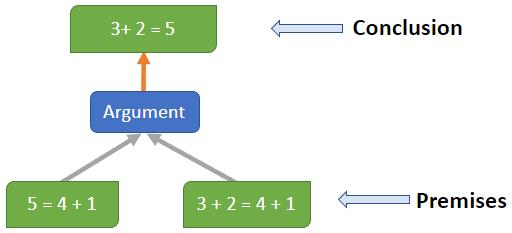
\includegraphics[height=3.5cm]{argument}}
\caption{An argument represented as a graph.}
\label{argument}
\end{center}
\end{figure}

A set of arguments can thus be represented as a single graph that we call an \textbf{argument graph} (Figure \ref{argument_graph}).

\begin{figure}[htbp]
\begin{center}
\fbox{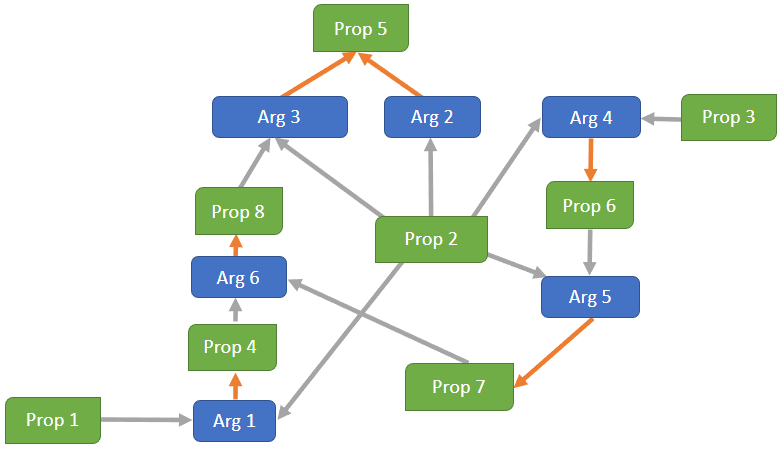
\includegraphics[height=7cm]{argument_graph}}
\caption{A set of arguments forming an argument graph.}
\label{argument_graph}
\end{center}
\end{figure}


\subsection{Generating Proof Graphs}
An argument graph along with a set of set of axioms results in a \textbf{proof graph}. Any reachability algorithm starting with the axiom nodes is sufficient to create the proof graph (See Figure \ref{proof_graph1}).


\begin{figure}[htbp]
\begin{center}
\fbox{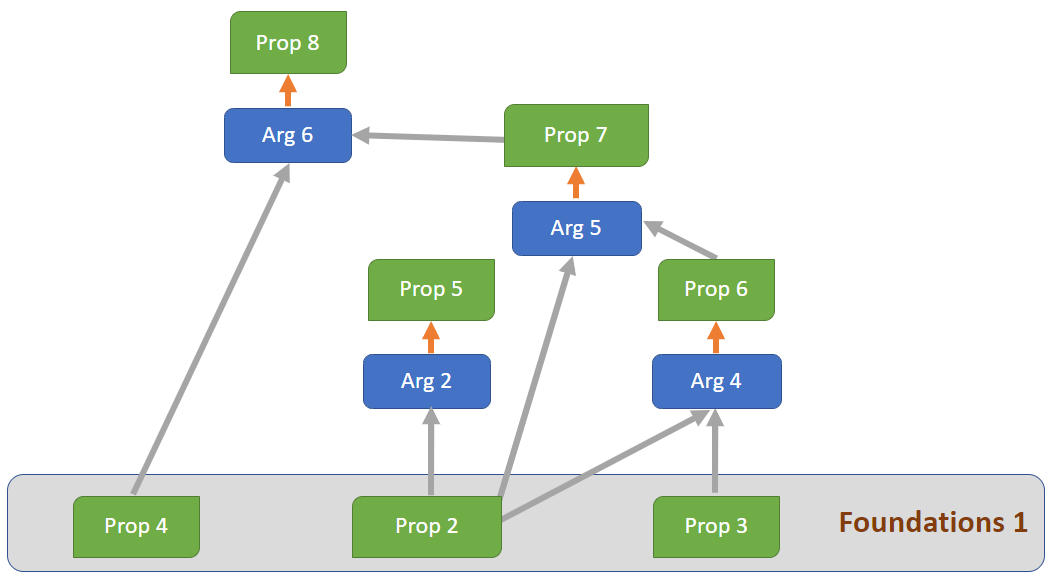
\includegraphics[height=7cm]{proof_graph1}}
\caption{Proof graph from argument graph (Figure \ref{argument_graph}) using `Prop 2', `Prop 3', Prop 4' are axioms.}
\label{proof_graph1}
\end{center}
\end{figure}


A proof graph is a directed acyclic graph and contains complete proofs (including all alternate proofs) for all its propositions.

\begin{figure}[htbp]
\begin{center}
\fbox{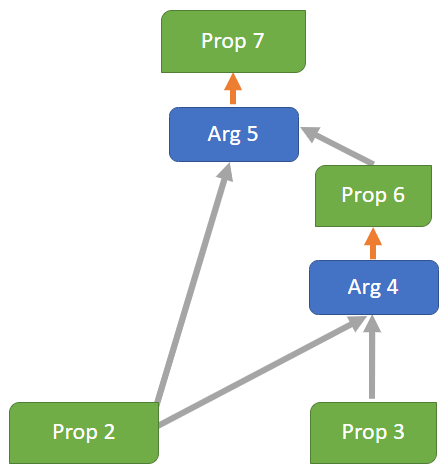
\includegraphics[height=6cm]{proof_prop7}}
\caption{Proof of `Prop 7' from proof graph in Figure \ref{proof_graph1} uses arguments `Arg 4' and `Arg 5'.}
\label{proof_prop7}
\end{center}
\end{figure}

Note that an argument graph combines with different sets of axioms to generate different proof graphs. The same argument may be utilized in multiple belief sets (Figure \ref{proof_graph2}).

\begin{figure}[htbp]
\begin{center}
\fbox{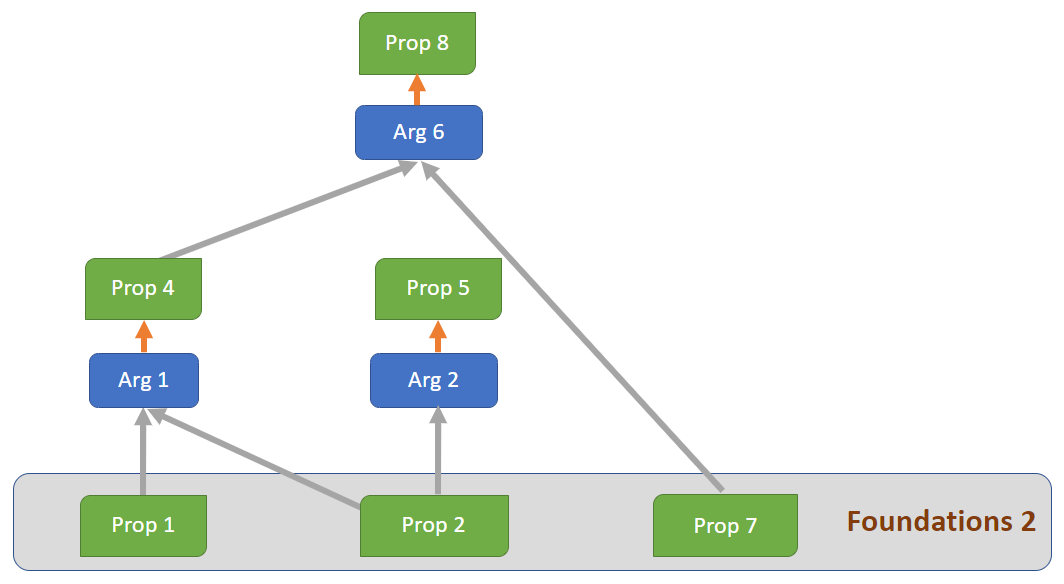
\includegraphics[height=8cm]{proof_graph2}}
\caption{Proof graph from the same argument graph (Figure \ref{argument_graph}) using `Prop 1', `Prop 2', and Prop 7' as axioms.}
\label{proof_graph2}
\end{center}
\end{figure}

\subsection{Validity of Arguments}

The correctness of proofs obtained by the above process is contingent on the validity of the arguments in the argument graph. The validity of an argument is, in principle, independent of other arguments and objectively verifiable. Formally defined logistic systems indeed have a mechanical procedure to independently verify validity of arguments.

However, only a small section of Mathematics is developed using formally verified arguments. Vast majority of mathematics is verified via peer review, some of this knowledge is curated by experts in books, encyclopaedias. The claim of validity of proofs (arguments) is judged based on the various parameters such as academic standing of the claimant, reputation of the peer reviewing journal, the history of errors of the book or encyclopaedia containing them, etc. Clearly, these criteria are subjective and each individual's criteria of accepting validity of an argument can vary to some extent.

Sophize doesn't promote or endorse any criteria. Instead, it allows its users to choose the criteria they believe in. The validity criterion is modelled as a proposition and is attached to arguments as a premise. 

\begin{figure}[htbp]
\begin{center}
\fbox{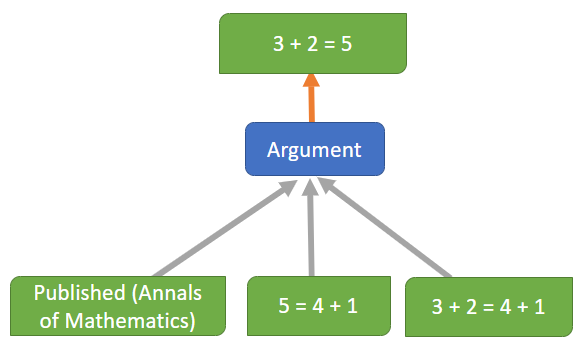
\includegraphics[height=5cm]{validity_criterion}}
\caption{Validity criteria as an argument premise.}
\label{validity_criterion}
\end{center}
\end{figure}

To easily manage validity criteria, the relationships between validity criteria are also maintained in the argument graph using argument-like dependency graphs. Eg. "Published in journal with SJR score $>$ 0.67" $\rightarrow$ "Published in Annals of Mathematics". By maintaining relationships like above, Sophize allows its users to conveniently choose multiple sources they consider to be reliable with a single manually chosen criterion. 

\subsection{Belief Sets}
\label{sec:bset}

A proposition is true if it is the conclusion of a valid argument and the premises of the argument are also true. Of course, this means that we need to start with some propositions that are assumed to be true without further justification. Traditionally, these are mathematical axioms and are considered to self-evidently true. In mathematical inquiry, theorems are proven/disproven in one or more multiple theories, each with its own set of axioms. Each theory may have its theoretical advantages and practical uses and there are no universal basis to choose one theory over another when trying to assert a proposition's truth/falsity.

Thus, Sophize allows any set of propositions to be considered true without evidence. Such a set of propositions is called a \textbf{belief set}. Propositions representing argument validity criteria are also part of belief sets. All propositions that are considered to be true in a belief set without proof are called its `unsupported propositions'. In addition, a belief set can also contain a number of `proof-generating machines' (e.g. for managing axiom-schemas) that will be discussed later. For ease of use, belief sets can also contain other belief sets.

The truth-value of a proposition is only defined within a belief set - there is no notion of of absolute or universal truth. Sophize creates proof graphs for all its belief sets.

\subsection{Tracking Inconsistencies}
If a proposition and its negation is proved within a belief set, it is inconsistent. As noted by the principle of explosion, any proposition can be proved from such a contradiction, thus making the claim of truth of any proposition practically worthless.

Thus, it is important to track and report contradictions in a belief set. To do that Sophize has a semantic notion of negation of a proposition. The premises or conclusion of an argument can be negations of propositions. When a proposition and its negation are proven, the system reports such contradictions for every belief set. When generating proof graphs from the argument graph, a contradicting proposition cannot be used a premise for any argument.

\subsection{Aggregating Knowledge}



\section{Proof-Generating Machines (PGM)}
\label{sec:pgm}
A lot of mathematical knowledge is computed. Computation machines (e.g. calculators, algebras) can be seen as performing the following tasks
\begin{itemize}
\item Parsing the input into a language that can represent math formulae. 
\item Finding and outputting an equivalent form of the formula.
\end{itemize}
Thus, their focus is not on finding the proof but only finding the equivalent (simplified) representation of the input formula (Although many computer algebras do show the steps of the computation.). With Sophize, the focus instead is to generate proofs of the input propositions. A \textbf{Proof-generating machine} (PGM for short) is a computer program that generates a partial proof graph against or in favour of an argument. PGMs can also have the capability to perform tasks 1 and 2, mentioned above.

PGMs take in some text as input which is parsed by the each PGM as they wish. Typically the text is treated either as a proposition (e.g. `3 + 5 = 8') or a formula (eg. `5+6') and in the latter case the PGM is responsible for finding an appropriate proposition (eg. `5 + 6 = 11') for the given input. The PGM then generates a proof graph for this proposition and returns back to the user.

The Sophize platform itself merely forwards the request to the associated PGM and performs some checks on the output returned. Any http server that can process a proof request can be easily plugged in to Sophize platform using its HTTP address. One server can implement multiple PGMs.

\subsection{`Active' PGMs}
As with other parts of Sophize, the validity of the output of a PGM is not taken for granted. Each PGM must specify all the propositions (premises) that it will use in the root nodes of the proof graph it returns. In addition, a PGM may also delegate parts of proofs to another PGM. These PGMs must also be specified. 

A PGM is considered `active' in a belief set iff:
\begin{enumerate}
\item all of its premises are true in the belief set.
\item all the PGMs it delegates-to are active.
\end{enumerate}

If the PGM returns a proof graph that utilizes As with an argument, one or more premises is used to indicate the validity of the PGM (Eg. tested by X, verified by some committee, another program etc). Thus, to be considered active in a belief set, the PGM must have a verification criteria that matches the belief set's requirements. The output of a PGM is not used in belief sets in which it is not active.

\subsection{PGM Response}
The response of a request to any PGM has the following components:

\begin{itemize}

\item Truth value, i.e., whether the PGM considers the input proposition (provided or computed) true or false. PGM can also indicate that it doesn't understand the input or prove/disprove the proposition.

\item Proof graph (or a subset of proof graph) generated by the PGM in favour or against the input proposition. This component is skipped if only computation results are requested.
\end{itemize}

Note that unlike other propositions and arguments on Sophize, these are not stored on disk. They have a temporary URI specified in a slightly different format. The leaves of the DAG can have two kinds of arguments:

\begin{enumerate}
\item Arguments whose the premises are limited to the premises of the PGM.
\item Special `Arguments' that indicate that the generation of the remaining proof must be delegated to another PGM. In case of large proofs, a PGM may also delegate to itself after generating some (say 100) arguments.
\end{enumerate}
\subsection{Materializing results}

Sophize allows saving the fact that a machine has returned a valid proof for a proposition (not the actual proof itself which can be quite large). Then this proposition can be used in further proofs without the need to invoke the proof generation every time. The proof, of course, can be requested by the users whenever required.


\section{Sophize Markdown}

In the author's view, it is crucial to maintain the proofs graphs for building trustable knowledge. However, the presentation of proofs as graphs to users is perhaps not very convenient. Traditional text based narration remains indispensable when presenting knowledge to the reader.

We have extended the Markdown language - a lightweight markup language for creating formatted text using a plain-text editor - for building a rich narration interface. It allows users to quickly encode and present semantic data, to show the truth status of propositions available in prose, and to effortlessly access proof graphs. 

With Sophize Markdown, we can easily add \LaTeX\space by enclosing it between two \$ signs (or \$\$ for display math). The detailed specification of Sophize Markdown is available here. Many of its features are demonstrated at: \url{https://youtu.be/5UYOpQwcjCk}. We highlight the prominent features here.

\subsection{Embedding semantic data}

With Sophize Markdown we can easily link resources such as terms, propositions, and arguments. Links can be added using the pound sign (\#) and the resource's URI. There are multiple resource link options that can be used for changing the behavior and text of the resource link. The following examples demonstrate these options.

\subsubsection*{Example 1}
\begin{verbatim}
#P_cosine_law|UC generalizes the #P_pythagorean for all kinds of #(T_triangle, 'triangles').
\end{verbatim}

\paragraph{The above code is rendered as:}
\begin{mdframed}
\dashuline{Law of cosines} generalizes the \dashuline{Pythagorean theorem} for all kinds of \dashuline{triangles}.
\end{mdframed}

The link options 'UC/LC' makes the link text upper-cased or lower-cased.

\subsubsection*{Example 2}
\begin{verbatim}
#T_matrix_multiplication|NO_LINK is a #(T_commutative_property, 'non-commutative'|NAV_LINK)
#T_binary_operation.
\end{verbatim}

\paragraph{The above code is rendered as:}
\begin{mdframed}
Matrix multiplication is a \underline{non-commutative} \dashuline{binary operation.}
\end{mdframed}
This example shows the various link behaviours. The first element shows `\#wiki/T\_matrix\_multiplication' on mouse-hover. The second link navigates the page to a different URL. Clicking on the third link pops up a modal dialog box like so:

\begin{figure}[htbp]
\begin{center}
\fbox{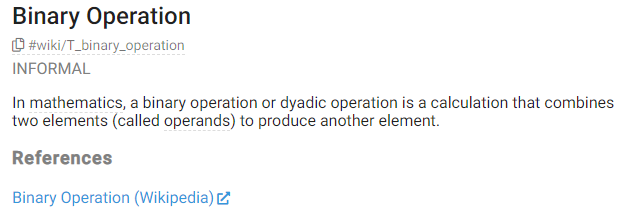
\includegraphics[height=5cm]{modal}}
\caption{Modal dialog box for the term binary operation. These boxes can also have content that uses all three types of links. }
\label{modal}
\end{center}
\end{figure}

\subsubsection*{Example 3}

\begin{verbatim}
# Conic section

A conic section (or simply conic) is a curve obtained as the intersection of the
surface of a #wiki/T_cone with a #wiki/T_plane. There are three types of conic sections.

## Ellipse
#oxford/T_ellipse|EXPAND #wiki/P_ellipse_area|EXPAND

## Parabola
...
\end{verbatim}

\paragraph{The above code is rendered as:}
\begin{mdframed}
\section*{Conic Section}
A conic section (or simply conic) is a curve obtained as the intersection of the surface of a \dashuline{cone} with a \dashuline{plane}. There are three types of conic sections.

\subsection*{Ellipse}
An ellipse is a regular \dashuline{oval} shape, traced by a point moving in a plane so that the sum of its distances from two other points is constant. The area $A_{ellipse}$ enclosed by an ellipse is $$A_{ellipse} = \pi a b$$where $a$ and $b$ are the lengths of the \dashuline{semi-major} and \dashuline{semi-minor} axes, respectively.

\subsection*{Parabola}
...

\end{mdframed}

In the above example, the `EXPAND' option expanded the definition of the term, and statement of the proposition in place. Thus we were able to easily re-use concepts and theorems already extracted from other sources (say, Wikipedia and the Oxford dictionary in this case).

\subsection{Truth Status}

Sophize markdown adds an icon next to each proposition link. This icon indicates whether the proposition has been proven or dis-proven (or both) in the currently selected belief set using a check-mark or a cross. Clicking on the icon brings up the proof graph as shown in Figure \ref{proof_tree}. If the users switches from one belief set to another, the icon is updated based on the truth values in the new belief set but other parts of the article are unchanged.

Similarly, an icon is added next to a proof generating machine which indicates whether the PGM is active or not.

\subsection{Formal Language Support}

In formal languages, definitions of terms, statements of propositions, and supporting argument text may be parse-able by an external parser. We can convert the externally parsed output into Markdown in such a case, where each term is automatically linked to the appropriate resource. This provides a convenient interface, where the user types in the native language, and the final output automatically allows users to explore all concepts that make up the input statement in depth. Currently, this is demonstrated in the use of Sophize Markdown with the Metamath language.

\begin{figure}[htbp]
\begin{center}
\fbox{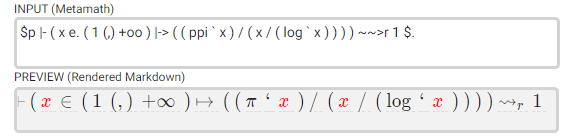
\includegraphics[height=3cm]{formal}}
\caption{The prime number theorem written in Metamath language and rendered as Markdown in real time.}
\label{formal}
\end{center}
\end{figure}


\section{Building a Modern Mathematics Library}
The argument and proof graphs in help us build a network of information that spans across a wide variety of sources (including live results from PGMs). Using different belief sets, users can view mathematical knowledge arising from different theoretical foundations and choose what they consider to be reliable. With Sophize Markdown, users can easily embed semantic information, thus making it convenient to explore the network of knowledge that is being built. However, a few more practical issues need to be overcome to build a modern scalable library with reliable information.

\subsection{Semantic Data Extraction}
Utilizing the full range of features offered by the Sophize platform requires the availability of semantic information. However, extracting semantic information from unstructured or semi-structured literature is a difficult problem. This problem can be seen as composed of several sub-problems:
\begin{itemize}
\item Finding definitions and propositions in prose.
\item Associating the appropriate entity with a term used in prose for quick lookup.
\item Identifying arguments and along with premises and conclusion.
\item \label{prob:dup} Identifying duplicate definitions and propositions used in different sources.
\end{itemize}

Solving these problems would need manual effort (e.g. crowd-sourcing) combined with automated extraction tools. Recent progress in machine learning and natural language processing techniques does make this problem seem tractable.

\subsubsection{}


\subsubsection{Connecting Across Datasets}
The sub-problem 4 mentioned above is crucial to help make connections across datasets. For example, once we have identified that the `Jensen's Inequaility' in a published paper is same as the Planetmath proposition with the same name, Planetmath's proof is made available to the reader of the published paper. 

\subsection{Search Interface}


\subsection{Data Management}
Sophize organizes 


\subsection{Collaboration}





\todo{copyright/access management}

\todo{efficient computation and storage of proof graphs}

\todo{ storing and reading data in disk/GitHub like repo }

With Sophize Markdown at its core, Sophize's collaboration interface\cite{todo}  (\underline{\href{https://youtu.be/d3gaalJ7UQM}{demo}}) is able to provide key features such as easy linking of existing math content, \LaTeX\space support, and live preview comment drafts.


\subsection{Connection across data sources}
\todo{What are Translations? (informal to formal, formal to other formal), Why do we need translations?}

There is no good way to claim equivalence of propositions across different formal systems. [Formal Harmony still in infancy, theory morphisms aren't yet practical].


Eg. ZFC (informal) + ZFC (metamath) + Jensen's Inequality (metamath) + validity criteria (translation feels right to metamath group) $\rightarrow$ 
Jensen's Inequality (informal)

But, we can represent translations manually using arguments. Such translations do not stand on a very firm foundation and that should be indicated in the validation criteria of the argument. Again, a user can choose not to accept such criteria. In that case, these translations will not be used in the generating proof graphs.


Thus we can create proof graphs that have arguments from different languages.

\subsection{Uses}
Efficiently modelling different axiomatic systems that have a large overlap of arguments(eg. euclidean/parabolic/hyperbolic geometry, ZF/ZFC etc)

Conjectural knowledge (Riemann hypothesis). 
Practical utility of conjectural knowledge - eg. a lot of information security systems assume "P is not NP"
Proof tailored to needs. Proof graph can be easily converted to prose too.


\subsubsection{Other Notes}
\todo{What criteria are met based on the 2013 report}

\todo{How much math can be represented. Eg. three valued logic}

\todo{Sophize's limitations. In "Potential Value of a
Digital Mathematics Library" in 2013 report. Sophize offers no way to more easily find analogies or weaker forms of reasoning like “If A is true, then B is true. B is true; therefore, A becomes more plausible.” }

\bibliographystyle{alpha} 

\bibliography{mybib}

\end{document}
